\documentclass{article}
\usepackage[utf8]{inputenc}
\usepackage{indentfirst}



\title{CSci 4511W TSP Project Final Report}
\author{Cho Zhang; Guanping Zhong}
\date{May 2019}

\usepackage{natbib}
\usepackage{graphicx}
\usepackage{nonfloat}
\usepackage{array}



\begin{document}

\maketitle


\begin{abstract}
This project explores TSP with a small-size data set (att48.tsp: US state capitals) and TSP with a large-size data set (ch130.tsp: 130 cities), using Genetic Algorithms with 100 generations (GA) and Ant Colony Algorithm (ACO) for both data sets. After gaining practical codes for the two algorithms and enough data, totally four kinds of experiments were conducted. GA was applied for att48.tsp and ch130.tsp respectively for 10 times. Also ACO was used for att48.tsp and ch130.tsp respectively for 10 times. Complete data was gathered to analyze their performances, and plots and tables were created to show the differences. Based on those, convincing conclusions can be drawn. 
\end{abstract}

\bigskip

\section{Introduction}
The project will be about Traveling Salesman Problem. We have a dream to have a road trip around the US, exploring as many cities as possible, using as little money as possible. We learned TSP problem from this AI class, which is a salesman wants to explore all cities on the map through the shortest path. We think it is very

interesting and want to apply it to deal with the above real-world problem.

As we are students, the budget for our travelling is limited. We want to make a plan in advance to find the cheapest route. To be specific, we consider the total expense for the fuel we consume during the trip as the overall cost. The algorithms choose a random city as the starting city. The goal we want to achieve will be finding out the cheapest routes to visit all other cities when starting from that city and coming back.

There are 48 capital cities in the US, which means the size could be like 47! computed in permutations. Regular algorithms can take a long time to get the optimal solution, so reducing time complexity will be one of the primary tasks for finding the optimal solution.

After searching some information, we found that for some large data sets it is hard to determine the optimal solution\cite{10.1007/978-3-642-13800-3_29}. However, it is very important to make a comparison when exploring a certain algorithm. Also, it is interesting to explore different datasets and see how it fits those search algorithms. Consequently we also choose another dataset called “ch130” as a comparison, which includes 130 cities’ position information. 130 is more than 48, but the number is not too big to cause too much time to run. 
After downloading some data sets from the internet, we can have access to distance values between every pair of cities. That way we can begin to explore the possible solutions for our road trips. 
According to the characteristics of different algorithms, we decided to implement generic algorithm and Ant Colony Optimization\citep{LiJ.2018APSA}. The reasons for choosing these two algorithms are specified in the background section below. In detail, we will run the two sets of codes for the two maps, which are ch130 and US. In the analysis, we will compare all the results from different conditions. We will look for the lowest cost and will also pay attention to the run-time and space complexity, thus figure out the better algorithm accordingly. 

\section{Background} 
As a classic example for unsolved NP problem, TSP is referred as a mathematical model at most times. Even though it has not been solved but various algorithms have been created to solve either the math model or the real-world problems. None of them is perfect, but when there is a specific problem, like how to generate a solution for traveling each city in different countries, it is possible to look for solutions to some degree. If we use a real country with hundreds of cities, we are supposed to consider the memory and runtime issue when searching for solutions. Even for small TSP with 10 cities, it could take a long time to get the results on computers. To start with, getting familiar with all the algorithms is necessary. The literature review below will be an overview of the field, with a focus on analyzing relatively the most helpful algorithms and how they can contribute to the project.

\section{Literature Review}
There are some pretty common algorithms which have been explored by researchers. For example, \citep{Vikas2017Raman}includes a review of three approaches used to solve TSP problem, which are genetic algorithm, colony optimization and particle swarm optimization. It analyzes their characteristics and advantages, including their development in the past few years. What is more, the authors also make comparisons among those algorithms. One of the conclusions is that different sizes of problems may need different approaches, and there is no such an algorithm that works always best for all problems all the time. It makes sense for this project as there will be a comparison of two datasets with different sizes, which are US capital cities and cities in ch130.

Similarly, in the book\citep{GutinGregory2007TTSP}, the author introduces some other useful methods in order to solve the TSP problem. There is an analysis of how those algorithms work through accurate computation, as well as how heuristic and metaheuristic algorithms can be applied. The book also listed a number of different versions of TSP problem, including bottleneck TSP, generalized TSP, prize collecting TSP, maximizing TSP and orienteering problem. It is practical for the project because it will be an interesting real-world version of TSP.

As a benchmark for combinatorial optimization, TSP can be solved by two main groups of algorithms. One of them is based on the energy minimization principle, and Hopfield neural networks were thought highly of as one method of this principle. However, it has not been put into practical use, and only the super computer can deal with it for even small-sized TSP, as stated in\citep{7175910} . At most of the time, Hopfield neural networks was referred as mathematical model, which makes it difficult to be implemented. In general, the cost for this method is too high, so it is not appropriate to be used for TSP.

The other group is heuristic algorithms, which is used more frequently. Acting more like a steepest descent algorithm, Tabu search is one instance of heuristic algorithms. According to\citep{SchneiderJohannesJosef2006TSAt}, it will use a tabu list to store all tabus which are the selected best neighboring configuration. Because the number of tabu will increase during the iteration, checking whether the neighboring configuration is the tabu takes a lot of time. If there is no good way to improve it, the Tabu algorithm will cost a large number of time and memory. Consequently it is also not a good way to solve the TSP problem for this ongoing project.

Genetic algorithm (GA) as a computational intelligence method is a search technique used in computer science to find approximate solutions to combinatorial optimization problems. Journal paper\citep{Kartik2014Rai} includes a general review of genetic algorithm. The authors paid attention to interesting examples of permutation problems similar to TSP, as well as some commonly used methodology in order to solve the problems. Through analyzing computational experiments and displaying data, genetic algorithm is emphasized significantly among all the approaches. What is more, it is stated that there are ten major steps in genetic search, and it also consists of encoding, evaluation, crossover, mutation and decoding process.

Genetic algorithm even show better performance after improvements. \citep{VahdatiG2009ANAt}focuses on avoiding premature convergence by increasing its speed. The main method proposed by the authors is utilizing a heuristic crossover and mutation operation to decrease the number of generations as much as possible, so that it will not be very easy to be trapped in loops when visiting all cities. It also means that the whole process of finding out the global optimal solution will be more efficient, using the algorithm presented in the paper. 

In the ongoing project, the number of cities in ch130 is larger than the US, so it is planned to be the bigger version of TSP. In that way, the slow and premature convergence are the most common problems and they cannot be solved easily. The paper\cite{ChenJie2011UGAB} introduces a new algorithm based on the hybrid probability distribution (EABHPD), where the area partition strategy can be used multiple times to get a good compromise result. Through dividing the whole TSP into several small TSPs, as well as using EABHPD and genetic algorithm, the large-scale TSP will be solved with faster convergence.

Ant Colony is another reasonable approach of the heuristic algorithm, and it is able to discover the solutions of TSP fast. \citep{LiJ.2018APSA}provides an improved algorithm based on ant colony optimization algorithm, using a negative feedback mechanism to enhance the accuracy of the shortest path. Based on the principle of pseudo-dynamic search, the pheromone concentration and the distances between cities will result in the inefficiency of ant colony search. It solves the TSP problem effectively and helps avoid the ant colony optimization algorithm jumping out a local optimum easily. Although it is a little hard to deal with the limitation, it is able to create practical results which can be very close to the real optimal solution, thus it is a good choice for the project to be done.

Actually there have been interesting TSP applications in natural environment. Paper\citep{FlipPhillips2010TTSP} from Journal of Vision lifts an interest of those applications. In the experiments for retrieving the solution, the authors used two different areas. The only difference between them was one was flat and open, and the other one was full of obstacles. There were fifteen marks representing fifteen cities in TSP. After careful tests, the researchers found the performances are obviously different for the two fields, shown in error percentages. That means, in the real world, the results of TSP actually depend on the natural environments to some degree. It analyzes results through computations and displays them in multiple figures. Considering this example, the ongoing project exploring cities in ch130 and US is even more meaningful. 

To summarize, heuristic algorithms will be used for the project. To be specific, there will be a comparison between Genetic Algorithm and Ant Colony algorithm. Both of them will be utilized for TSP in US and ch130. The different performances will reveal that which one will fit better for small-size or large-scale TSP.


 

\section{Experiment Process}
The approach used in this project is running Genetic Algorithm and Ant Colony Algorithm respectively for cities in ch130 and US, trying to figure out which one is better. Then comparing the cost of their shortest paths is supposed to show a general idea of their advantages and disadvantages under different conditions. 

The steps are below, in detail:

1. Searched codes for Genetic Algorithm and Ant Colony Algorithm, and picked a reasonable one for them correspondingly. Downloaded them for future use. The language utilized here is Python. The source codes are from\citep{gacode} and \citep{acocode}. For the Ant Colony Algorithm, there is no plotting function, so it is necessary to add one. It was not hard to get the positions of the points in order they were visited in the shortest path, so that what should be done was to loop through those points and connect them using a line. The created plots are allocated in the results section.

2. Searched database at\citep{database}, and obtained data of relative coordinates for cities in ch130 and US. The number of cities in ch130 is 130, and that for the US is 48. There are more cities in ch130, but the magnitudes of distances are much smaller than the US. It makes them distinguishable from each other.
To be specific, taking the example of ch130, the representation is like below:

 \begin{figure}[h]
  \begin{center}
    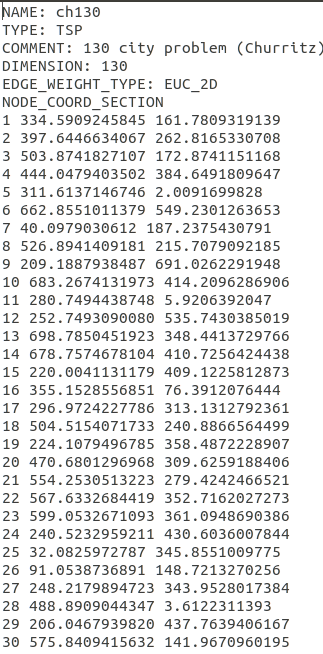
\includegraphics[scale=0.53]{image4}
  \end{center}
  \caption{CH130 TSP Data}
\end{figure}

\bigskip

The original data obtained from the website has lines of descriptions at the beginning of the file, followed by the numbers. The description includes the name of the file, the amount of lines of data, the type of the data, and so on. They help a lot to understand the basic situation of the data. However, when importing the data to the algorithms, these descriptions should be carefully handled, as the real data parts are what to be cared about in this project. On the other hand, some information such as the number of rows could be utilized to indicate some characteristics of the data.


The final readable file can include an N*N matrix that stores the distances between every two cities in TSP. However, a large scale of cities in the matrix means there needs to be much more blocks to store the information. It is also hard to read data like this and it will take lots of time. If using the matrix to store the distance information, the space in need would be N*N. 
Actually, the distance information can be mapped into the position, using Cartesian formula to calculate the distances rather than storing them directly \citep{database}, and it could reduce the memory used significantly. Nevertheless, mapping the distance to the position is not easy. For example, the first city could be an arbitrary point on x,y axis, and the second city can be another arbitrary point on the circle boundary of which the radius is the distance between the cities and the center is the position of the first city. But the third city's position can be “flipped” about the line connecting city one and two. To remove this kind of singularity, DISTANCETOPOSITION function is used in the TSPLIB\citep{datafunction}.

Adjusting the algorithms got from the first step is necessary, in order to make them work for the data. More specifically, applied practical functions to read the data from a file. For example, if the data is .txt type, readlines() can be used. For each record as a string, it also needs to be split into multiple float numbers, which represent relative coordinates of cities. Another point that needs attention is that sometimes not all content in the file is necessary, as there may be English words which should be dealt with differently with numbers. In short, both algorithms and data were adjusted in some way, so that they could match each other. 
In addition to importing the data, there should also be adjusted parts for exporting the results after running the algorithms. Printing the statistics such as the miles of the shortest path can be a good choice, especially when keeping updating it in the process. So it is easy to know how the result changes when utilizing different methods. What is more, based on the characteristic of Python, drawing the path is another good option. That way the consequences could be shown more vividly, which makes it easier for the comparison step.

\bigskip
3. Compared the results of the plots and statistics, and analyzed their similarities and differences. Basically the aspects of comparisons are like below:

(1). The magnitudes of the shortest path

In order to make the problems look easier, it is assumed that the cost for each distance unit is 1, which means the values of cost are equal to the values of distance of the path. Consequently, during the process of improving algorithms, not a lot of extra work needs to be added for that part. Printing out the digital numbers resulting from different algorithms and different city maps, and even putting them together in tables are the main methods of comparisons, which are clear and easy to understand. 

(2). The time used to finish the search

During the experiments, the time spent for running the codes are recorded. The speed depends on the languages in use as well as the  specific algorithms structures. Also, the situations of data are essential, as both the size of data and the magnitudes will influence the time taken for the calculation and exploration. Based on comparing the time needed for looking for a relatively shortest path to visit all the cities, it is possible to get a clue of the quality of the performances of different algorithms under different conditions. 

(3). The shape and size of the path 

According to the drawn plots, it is easy to compare paths under different conditions. It is possible to find out some similarities and obvious differences from viewing those plots directly. In general the more crossing the lines have, the longer the distance is. Below is an instance:

\bigskip
\begin{figure}[h]
  \begin{center}
    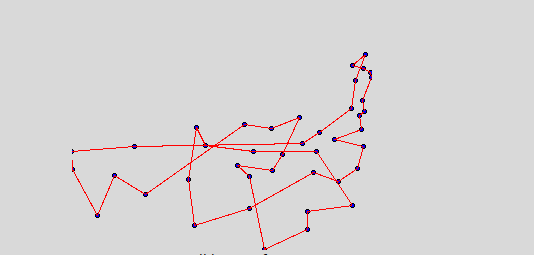
\includegraphics[scale=0.6]{image2}
  \end{center}
  \caption{Picture to show the example result}
\end{figure}
\bigskip

(4). The Standard Deviation 

Known as the most famous NP problem, TSP could not be solved in polynomial time. So the same algorithm would generate different results when run at different times. The standard deviation represents the stability of the algorithm which will be another attribute used to test the optimality to some extent.

\section{Experiment Result}
Basically, the design of the experiments includes running the two types of codes for different city maps. As both of the algorithms randomly try some directions or values and keep exploring the best results so far, every time the consequences are different. Thus there are ten trials in total, in order to make the conclusions more regular and meaningful. repeating each of them ten times. The printed results contain the magnitudes of the shortest paths, as well as the corresponding plots of the shortest paths. To be specific, the steps are like below, together with pictures showing results:

\bigskip
1. Apply the data set of US capital cities, and implement Genetic Algorithm for it. Record result data and the plot of the path. Repeat the action for ten times. The plot below shows one example of the ten trials. 



\bigskip
\begin{figure}[h]
  \begin{center}
    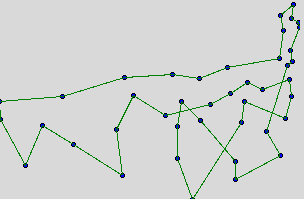
\includegraphics[scale=0.7]{image1}
  \end{center}
  \caption{Route visualization for using Genetic Algorithm on att48}
\end{figure}
\bigskip



2. Apply the dataset of main cities in ch130, and implement Genetic Algorithm for it. Record result data and the plot of the path. Repeat the action for ten times. The plot below shows one example of the ten trials. 

\bigskip
\begin{figure}[h]
  \begin{center}
    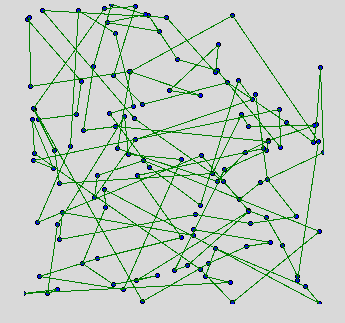
\includegraphics[scale=0.65]{image6}
  \end{center}
  \caption{Route visualization for using Genetic Algorithm on ch130}
\end{figure}
\bigskip

3. Apply the dataset of US capital cities, and implement Ant Colony Algorithm for it. Record result data and the plot of the path. Repeat the action for ten times. The plot below shows one example of the ten trials.


\bigskip
\begin{figure}[h]
  \begin{center}
    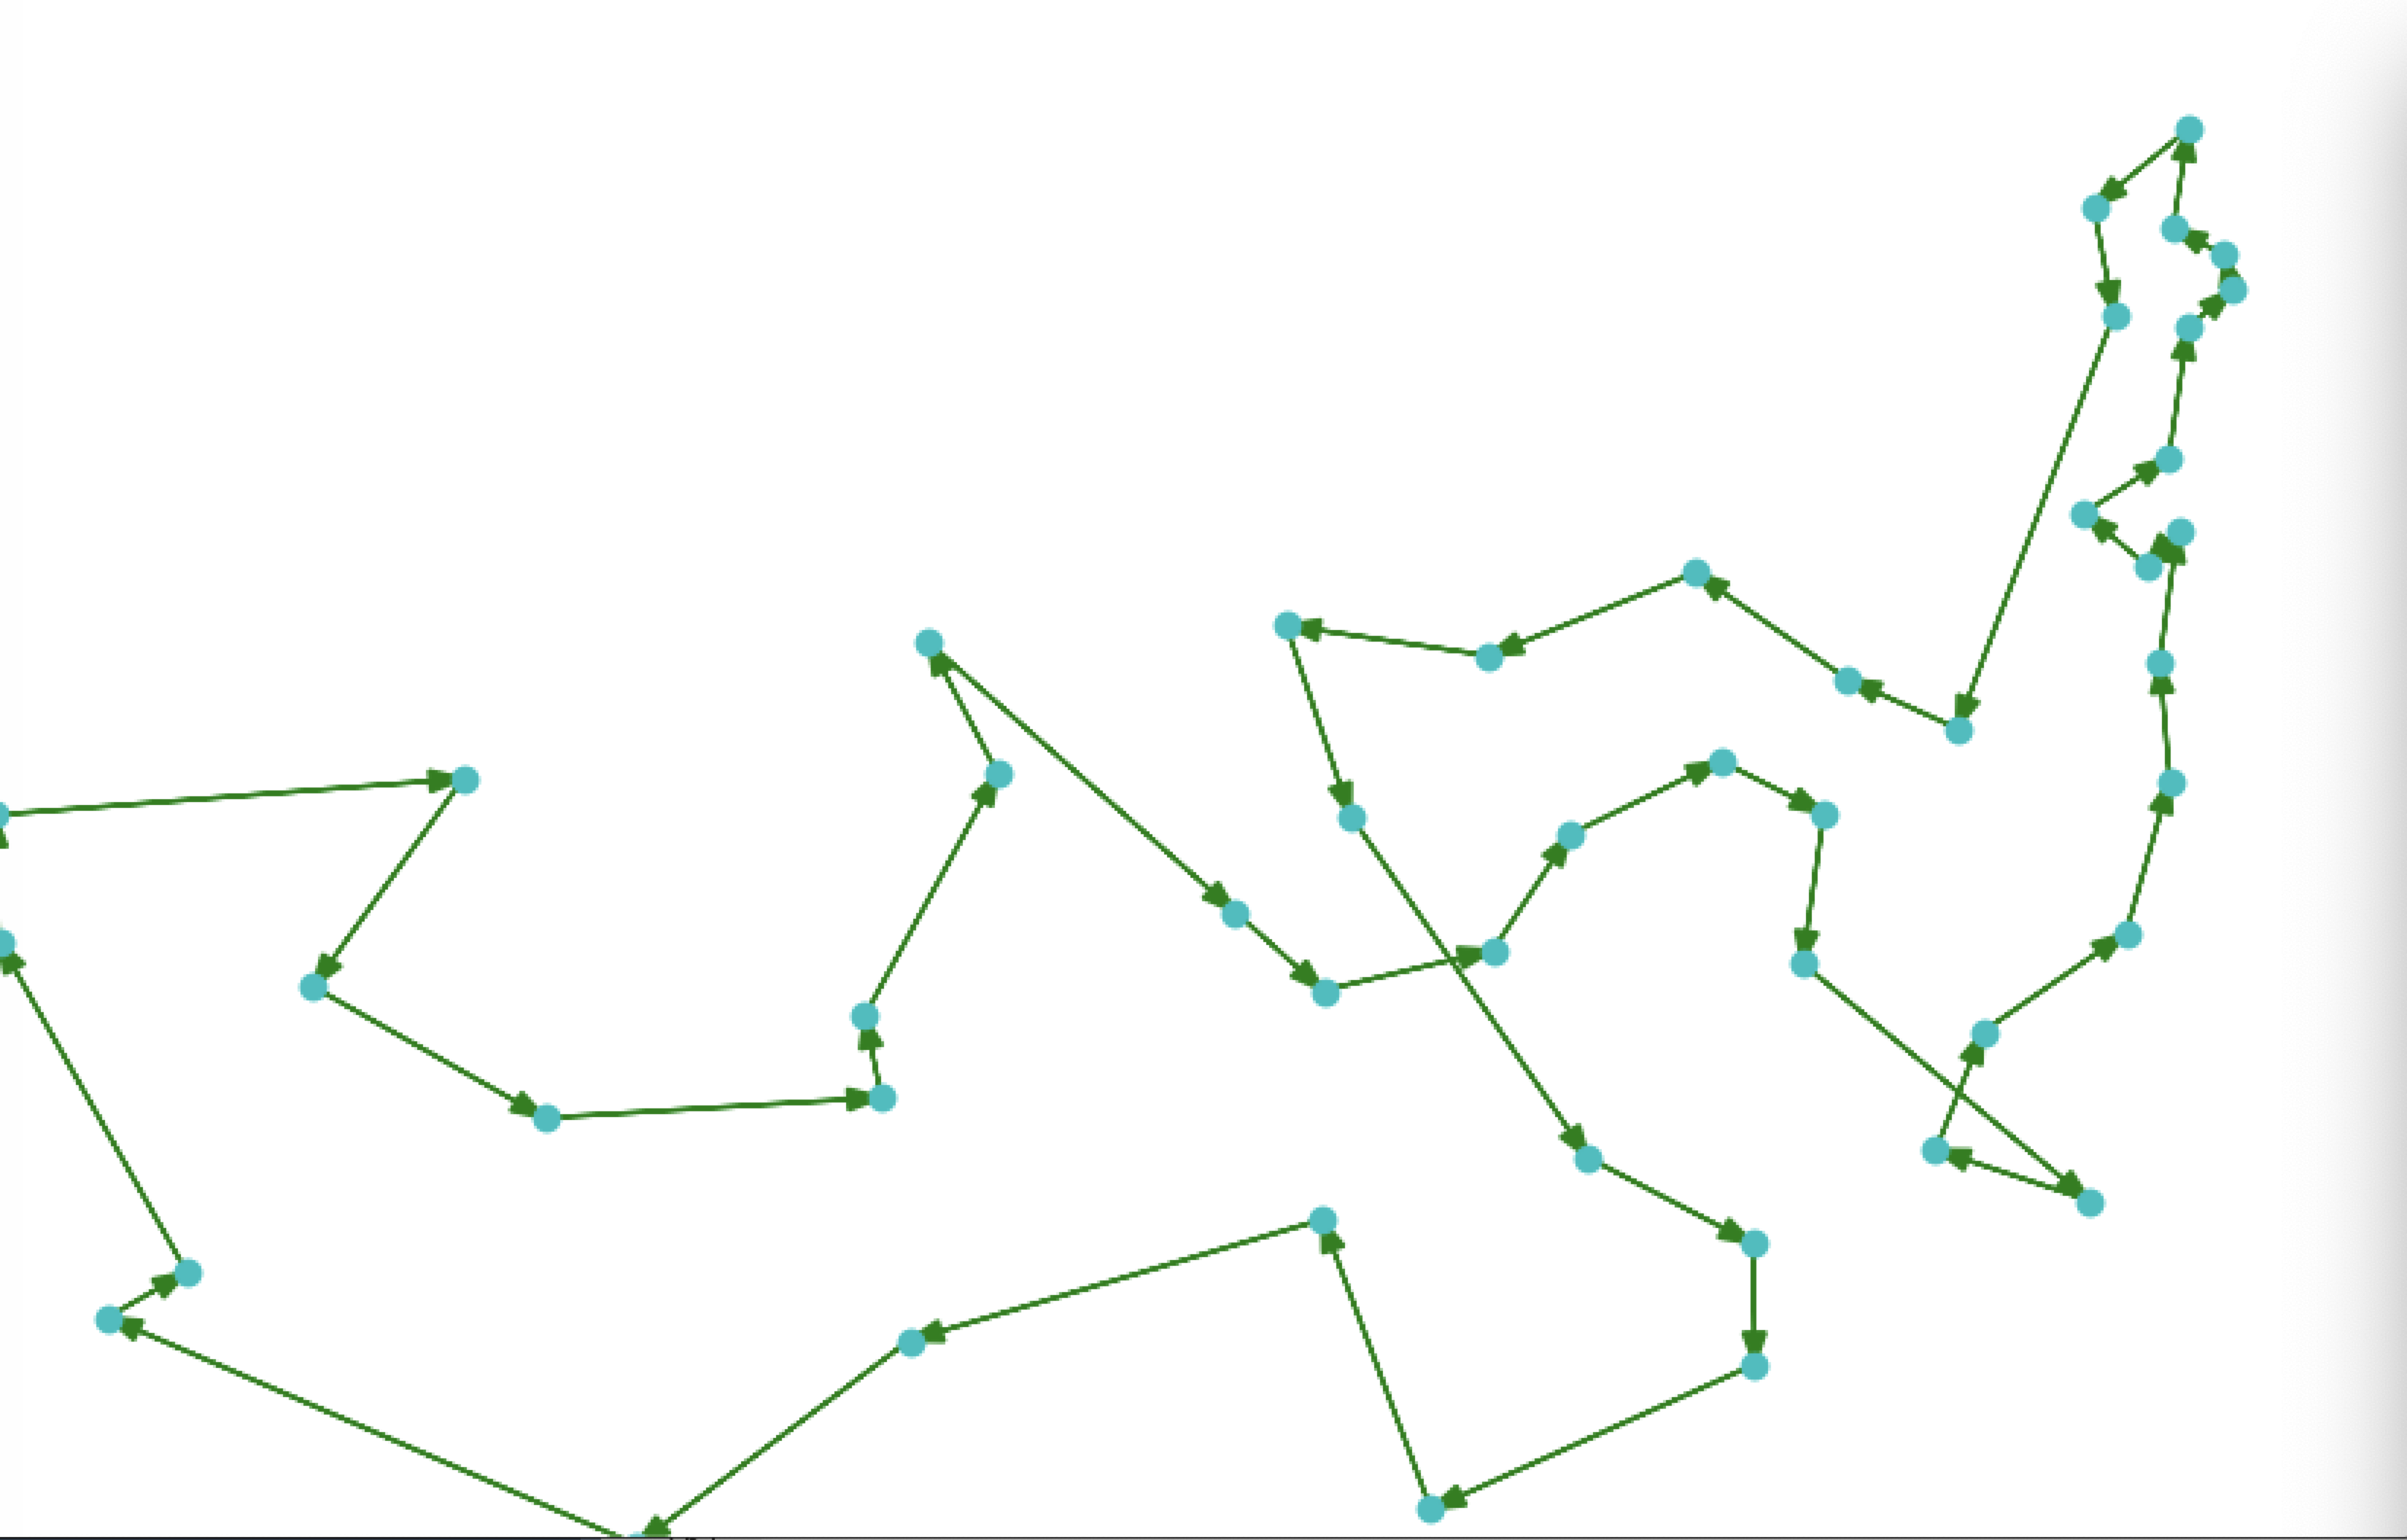
\includegraphics[scale=0.16]{image7}
  \end{center}
  \caption{Route visualization for using Ant Colony Algorithm on att48}
\end{figure}
\bigskip


4. Apply the dataset of main cities in ch130, and implement Genetic Algorithm for it. Record result data and the plot of the path. Repeat the action for ten times. The plot below shows one example of the ten trials.  

\bigskip
\begin{figure}[h]
  \begin{center}
    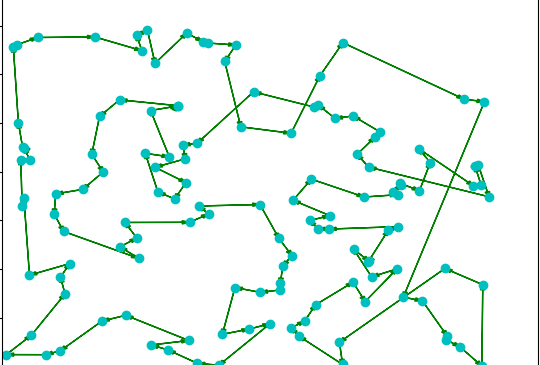
\includegraphics[scale=0.49]{image3}
  \end{center}
  \caption{Route visualization for using Ant Colony Algorithm on ch130}
\end{figure}
\bigskip


\section{Analysis}
Based on the results obtained from the last step, it is not difficult to collect all of them and put them into tables. That way the different performances could be easy to compare. For Genetic Algorithm, the generation time is 100. The attributes in the comparisons are average times used to complete the search, the average relative distance of the shortest paths, and the standard deviation of the two categories as well. For the time, although it can vary on different machines, it can be a variable used to see the general performance of the codes, as they were run on the same lab machine around the same time. There are four types of comparisons in total, and each one with only one different condition, which follows rules of the control variate method. 

\bigskip
1. Cities in ch130 and the US, both using Genetic Algorithm. 

\begin{center}
    Table 1: ch130 - Genetic
\end{center}

\begin{center}

\resizebox{.7\linewidth}{!}{%
\begin{tabular}{llllll}
\cline{1-3}
\multicolumn{1}{|c|}{}                   & \multicolumn{1}{c|}{Time} & \multicolumn{1}{c|}{Relative distance} &  &  \\ \cline{1-3}
\multicolumn{1}{|c|}{Average}            & \multicolumn{1}{c|}{37.2} & \multicolumn{1}{c|}{21423.8}           &  &  \\ \cline{1-3}
\multicolumn{1}{|c|}{Standard Deviation} & \multicolumn{1}{c|}{1.4}  & \multicolumn{1}{c|}{1377.3}            &  &  \\ \cline{1-3}
                                         &                           &                                        &  & 

\end{tabular}}

\begin{center}
    Table 2: US - Genetic
\end{center}

\resizebox{0.7\linewidth}{!}{%
\begin{tabular}{lllll}
\cline{1-3}
\multicolumn{1}{|c|}{}                   & \multicolumn{1}{c|}{Time} & \multicolumn{1}{c|}{Relative distance} &  &  \\ \cline{1-3}
\multicolumn{1}{|c|}{Average}            & \multicolumn{1}{c|}{2.4}  & \multicolumn{1}{c|}{43879.2}           &  &  \\ \cline{1-3}
\multicolumn{1}{|c|}{Standard Deviation} & \multicolumn{1}{c|}{0.2}  & \multicolumn{1}{c|}{4727.9}            &  &  \\ \cline{1-3}
                                         &                           &                                        &  & 
\end{tabular}}
\end{center}

The average distance of the shortest path for ch130 is obviously shorter than that of the US, and it is like half of the latter. And the former one has a smaller standard deviation, which means it is more stable. The average time spent for ch130 is much more than the US, but their standard deviations are similar.

\bigskip
2. Cities in ch130 and the US, both using Ant Colony Algorithm.

\begin{center}
    Table 3: ch130 - Ant Colony
\end{center}
\begin{center}
\resizebox{0.7\linewidth}{!}{%
\begin{tabular}{lllll}
\cline{1-3}
\multicolumn{1}{|c|}{}                   & \multicolumn{1}{c|}{Time}   & \multicolumn{1}{c|}{Relative distance} &  &  \\ \cline{1-3}
\multicolumn{1}{|c|}{Average}            & \multicolumn{1}{c|}{81.9} & \multicolumn{1}{c|}{7717.9}          &  &  \\ \cline{1-3}
\multicolumn{1}{|c|}{Standard Deviation} & \multicolumn{1}{c|}{1.8}  & \multicolumn{1}{c|}{131.1}           &  &  \\ \cline{1-3}
                                         &                             &                                        &  & 
\end{tabular}}

\begin{center}
    Table 4: US - Ant Colony
\end{center}
\resizebox{0.7\linewidth}{!}{%
\begin{tabular}{lllll}
\cline{1-3}
\multicolumn{1}{|c|}{}                   & \multicolumn{1}{c|}{Time} & \multicolumn{1}{c|}{Relative distance} &  &  \\ \cline{1-3}
\multicolumn{1}{|c|}{Average}            & \multicolumn{1}{c|}{12.0} & \multicolumn{1}{c|}{37564.5}           &  &  \\ \cline{1-3}
\multicolumn{1}{|c|}{Standard Deviation} & \multicolumn{1}{c|}{0.4}  & \multicolumn{1}{c|}{478.7}             &  &  \\ \cline{1-3}
                                         &                           &                                        &  & 
\end{tabular}}
\end{center}

The distance of the shortest path for ch130 is obviously shorter than that of the US, and it is like one fifth of the latter. And the former one has a smaller standard deviation, which means it is more stable. The average time spent for ch130 is much more than the US, but their standard deviations are similar.

\bigskip
3. Cities in ch130, using Ant Colony and Genetic Algorithm. 

\begin{center}
    Table 5: Ch130 - Ant Colony
\end{center}
\begin{center}
\resizebox{0.7\linewidth}{!}{%
\begin{tabular}{lllll}
\cline{1-3}
\multicolumn{1}{|c|}{}                   & \multicolumn{1}{c|}{Time}       & \multicolumn{1}{c|}{Relative distance} &  &  \\ \cline{1-3}
\multicolumn{1}{|c|}{Average}            & \multicolumn{1}{c|}{81.9} & \multicolumn{1}{c|}{7717.9}          &  &  \\ \cline{1-3}
\multicolumn{1}{|c|}{Standard Deviation} & \multicolumn{1}{c|}{1.8}      & \multicolumn{1}{c|}{131.1}           &  &  \\ \cline{1-3}
                                         &                                 &                                        &  & 
\end{tabular}}

\begin{center}
    Table 6: ch130 - Genetic
\end{center}
\resizebox{0.7\linewidth}{!}{%
\begin{tabular}{lllll}
\cline{1-3}
\multicolumn{1}{|c|}{}                   & \multicolumn{1}{c|}{Time} & \multicolumn{1}{c|}{Relative distance} &  &  \\ \cline{1-3}
\multicolumn{1}{|c|}{Average}            & \multicolumn{1}{c|}{37.2} & \multicolumn{1}{c|}{21423.8}           &  &  \\ \cline{1-3}
\multicolumn{1}{|c|}{Standard Deviation} & \multicolumn{1}{c|}{1.4}  & \multicolumn{1}{c|}{1377.3}            &  &  \\ \cline{1-3}
                                         &                           &                                        &  & 
\end{tabular}}
\end{center}

The distance of the shortest path using Ant Colony is obviously shorter than that of Genetic Algorithm, and it is like two fifths of the latter. And the former one has a smaller standard deviation, which means it is more stable. The average time spent for Ant Colony Algorithm is more than Genetic Algorithm, but their standard deviations are similar on average. 

\bigskip
4. Cities in the US, using Genetic Algorithm and Ant Colony. 

\begin{center}
    Table 7: US - Ant Colony
\end{center}
\begin{center}
\resizebox{0.7\linewidth}{!}{%
\begin{tabular}{lllll}
\cline{1-3}
\multicolumn{1}{|c|}{}                   & \multicolumn{1}{c|}{Time} & \multicolumn{1}{c|}{Relative distance} &  &  \\ \cline{1-3}
\multicolumn{1}{|c|}{Average}            & \multicolumn{1}{c|}{12.0} & \multicolumn{1}{c|}{37564.5}           &  &  \\ \cline{1-3}
\multicolumn{1}{|c|}{Standard Deviation} & \multicolumn{1}{c|}{0.4}  & \multicolumn{1}{c|}{478.7}             &  &  \\ \cline{1-3}
                                         &                           &                                        &  & 
\end{tabular}}

\begin{center}
    Table 8: US - Genetic
\end{center}
\resizebox{0.7\linewidth}{!}{%
\begin{tabular}{lllll}
\cline{1-3}
\multicolumn{1}{|c|}{}                   & \multicolumn{1}{c|}{Time} & \multicolumn{1}{c|}{Relative distance} &  &  \\ \cline{1-3}
\multicolumn{1}{|c|}{Average}            & \multicolumn{1}{c|}{2.4}  & \multicolumn{1}{c|}{43879.2}           &  &  \\ \cline{1-3}
\multicolumn{1}{|c|}{Standard Deviation} & \multicolumn{1}{c|}{0.2}  & \multicolumn{1}{c|}{4727.9}            &  &  \\ \cline{1-3}
                                         &                           &                                        &  & 
\end{tabular}}
\end{center}

The distance of the shortest path using Ant Colony is shorter than that of Genetic Algorithm, but without a lot of differences. And the former one has a smaller standard deviation, which means it is more stable. However, the time used to complete the search for Ant Colony Algorithm is more than for the US, but their standard deviations are similar.

\section{Conclusion}
The original problem explored in this project is to find out one or more most useful algorithm(s) that work for different sizes of TSP. Based on the experiment results and the analysis in the previous sections, there are some conclusions.
Generally speaking, Ant Colony Algorithm is usually slower than Genetic Algorithm with 100 generations, as the time spent to get the shortest paths using Ant Colony Algorithm are always more than that using Genetic Algorithm. However, it can get better results usually. It is able to find shorter paths than Genetic Algorithm, and it is more stable. The experiment data shows that there are obvious differences between the distances of the shortest paths when applying the two algorithms, and the Ant Colony Algorithm always get a shorter distance. 

Ch130 has more cities than the US, so it is reasonable that it takes more time to search the shortest path. However, the absolute values of distances for cities in ch130 are much smaller, which leads to the relative distance for the whole path being shorter. From the table comparing two algorithms used for ch130, it is easy to see that the average of the shortest paths generated by Ant Colony Algorithm is almost one third of that by Genetic Algorithm, and the time taken by the former one is about two times of the latter. Consequently, when time is not a significant factor that needs to be considered, Ant Colony Algorithm should be a better choice than Genetic Algorithm to work for data sets with large numbers of points. 

The US cities have larger magnitudes, but the number of points are much less than ch130. When comparing the results of two algorithms used for US capital cities, the average distance of the shortest paths using Ant Colony Algorithm is smaller than that using Genetic Algorithm, but only by 15\%, which is not a lot of difference. However, the time used by Genetic Algorithm is much less than Ant Colony Algorithm, by about one sixth. As a result, if time is an important element to deal with a certain TSP, Genetic Algorithm can be a more practical choice to deal with small-size TSP, which has less points to visit.

\pagebreak


\bibliographystyle{plain}
\bibliography{references}
\end{document}
